\documentclass[12pt,a4paper]{book}

\usepackage{amsmath}
\usepackage{amssymb}
\usepackage{tikz}
\usepackage[siunitx]{circuitikz}
\usepackage{emptypage}
\usepackage{IEEEtrantools}

\usetikzlibrary{scopes}

\pagestyle{plain}

\title
	{
	\huge The IPhO Compendium\\
	\large A Collection of Problems Presented\\ in The International Physics Olympiads
	} 
\date{}

\begin{document}
\maketitle
\frontmatter
\tableofcontents
\mainmatter
\chapter*{I IPhO (Warsaw, 1967)}
\addcontentsline{toc}
{chapter}{I IPhO (Warsaw, 1967)}
\section*{Theoretical problem}
	\subsection*{Problem 1}
	A small ball with mass $M=0.2\text{kg}$ rests on a vertical column with height $h=5\text{m}$. A bullet with mass $m=0.01\text{kg}$, moving with velocity $v_0=500\text{ms}^{-1}$, passes horizontally through the center of the ball. The ball reaches the ground at a distance $s=20\text{m}$. Where does the bullet reach the ground? What part of the kinetic energy of the bullet was converted into heat when the bullet passed through the ball? Neglect resistance of the air, the size of the ball and the bullet. Assume that $g=10\text{m}\text{s}^{-2}$.\\ \\
	\textbf{Solution}\\
	\begin{figure}[!hbtp]
	\centering
	\begin{tikzpicture}
		\draw (0,0) -- (12,0);
		\draw (1.05,0) -- (1.05,1.85) --(0.95,1.85) -- (0.95,0);
		\fill[red] (0.1,2) circle (0.1);
		\draw (0.1,2.4) node {$m,v_0$};
		\draw[->] (0.1,2) -- (0.5,2);
		\fill[blue] (1,2) circle (0.15);
		\draw (1,2.4) node {$M$};
		\draw[<->] (0.75,0) -- (0.75,2);
		\draw (0.5,1) node {$h$};
		\draw[densely dotted] (1,2) parabola (3,0);
		\draw[densely dotted, blue] (2.92,0.15) circle (0.15);
		\draw[<->] (1,-0.25) -- (3,-0.25);
		\draw (2,-0.5) node {$s$};
		\draw[densely dotted] (1,2) parabola (11,0);
		\draw[densely dotted, red] (10.75,0.1) circle (0.1);
		\draw[<->] (1,-0.10) -- (11,-0.10);
		\draw (6,-0.35) node {$d$};
	\end{tikzpicture}
	\caption{Sketch for Problem 1}
	\label{sketch_1}
	\end{figure}\par
	We will use notation shown in Figure \ref{sketch_1}.\par
	As no horizontal force acts on the system ball and bullet, the horizontal component of momentum of this system before collision and after collision must be the same,
	\begin{equation*}
		mv_0=mv^{'}+MV
	\end{equation*}
	where $v^{'}$ and $V$ are horizontal component of the velocity of the bullet and of the ball after collision, respectively.\par
	So,
	\begin{equation*}
		v=v_0-\frac{M}{m}V
	\end{equation*}
	From conditions described in the text of the problem it follows that
	\begin{equation*}
		v>V
	\end{equation*}
	After collision, both the ball and the bullet continue a free motion in the gravitational field with initial horizontal velocities $v$ and $V$, respectively. Motion of the ball and motion of the bullet are continued for the same time,
	\begin{equation*}
		t=\sqrt{\frac{2h}{g}}
	\end{equation*}
	It is the time of free fall from height $h$.\par
	The distances passed by the ball and bullet during time $t$ are
	\begin{equation*}
		s=Vt\text{ and }d=vt
	\end{equation*}
	respectively. Thus,
	\begin{equation*}
		V=s\sqrt{\frac{g}{2h}}
	\end{equation*}
	Therefore,
	\begin{equation}
		d=v_0\sqrt{\frac{2h}{g}}-\frac{M}{m}s
	\end{equation}
	Numerically,
	\begin{equation*}
		d=100\text{m}
	\end{equation*}
	The total kinetic energy of the system was equal to the initial kinetic energy of the bullet,
	\begin{equation*}
		E_0=\frac{mv_0^{2}}{2}
	\end{equation*}
	Immediately after the collision, the total kinetic energy ot the system is equal to the sum of the kinetic energy of the bullet and the ball,
	\begin{equation*}
		E_m=\frac{mv^{2}}{2}\text{ and }E_M=\frac{MV^{2}}{2}
	\end{equation*}
	Their difference, converted into heat, was
	\begin{equation*}
		\Delta E=E_0-(E_m+E_M)
	\end{equation*}
	It is the following part of the initial kinetic energy of the bullet,
	\begin{equation*}
		p=\frac{\Delta E}{E_0}=1-\frac{E_m+E_M}{E_0}
	\end{equation*}
	By using expressions for energies and velocities (quoted earlier) we get
	\begin{equation}
		p=\frac{M}{m}\frac{s^2}{v_0^2}\frac{g}{2h}\Big(2\frac{v_0}{s}\sqrt{\frac{2h}{g}}-\frac{M+m}{m}\Big)
	\end{equation}
	Numerically,
	\begin{equation*}
		p=92.8\text{\%}
	\end{equation*}
	\subsection*{Problem 2}
	Consider an inf\mbox{}inite network consisting of resistors (resistance of each of them is $r$) as shown in Figure \ref{sketch_2}. Find the resultant resistance $R_{AB}$ between points A and B.\\
	\begin{figure}[!hbtp]
	\centering
	\begin{circuitikz}
		\draw (-0.5,2.5) node {A};
		\draw (0,2.5) to[R, l=$\SI{}{r}$] (2.5,2.5) to[R, l=$\SI{}{r}$] (5,2.5) to[R, l=$\SI{}{r}$] (7.5,2.5) -- (8,2.5);
		\draw[dotted] (8,2.5)-- (9,2.5);
		\draw (2.5,0) to[R, l=$\SI{}{r}$] (2.5,2.5);
		\draw (5,0) to[R, l=$\SI{}{r}$] (5,2.5);
		\draw (7.5,0) to[R, l=$\SI{}{r}$] (7.5,2.5);
		\draw (-0.5,0) node {B};
		\draw (0,0) -- (8,0);
		\draw[dotted] (8,0) -- (9,0);
	\end{circuitikz}
	\caption{Sketch for Problem 2}
	\label{sketch_2}
	\end{figure}\\ \\
	\textbf{Solution}\\
	It is easy to remark that after removing the left part of the work, shown in Figure \ref{sketch_2_1} with the red square, then we receive a network that is identical with the initial network (it is result of the fact that the network is inf\mbox{}inite).
	\begin{figure}[!hbtp]
		\centering
		\begin{circuitikz}
			\draw (-0.5,2.5) node {A};
			\draw (0,2.5) to[R, l=$\SI{}{r}$] (2.5,2.5) to[R, l=$\SI{}{r}$] (5,2.5) to[R, l=$\SI{}{r}$] (7.5,2.5) -- (8,2.5);
			\draw[dotted] (8,2.5)-- (9,2.5);
			\draw (2.5,0) to[R, l=$\SI{}{r}$] (2.5,2.5);
			\draw (5,0) to[R, l=$\SI{}{r}$] (5,2.5);
			\draw (7.5,0) to[R, l=$\SI{}{r}$] (7.5,2.5);
			\draw (-0.5,0) node {B};
			\draw (0,0) -- (8,0);
			\draw[dotted] (8,0) -- (9,0);
			\draw[red] (0.5,-0.75) -- (3,-0.75) -- (3,3.25) -- (0.5,3.25) -- (0.5,-0.75); 
		\end{circuitikz}
		\caption{Auxiliary sketch for Problem 2}
		\label{sketch_2_1}
	\end{figure}\par
	Thus, we may use the equivalence shown graphically in Figure \ref{sketch_2_2}.
	\begin{figure}[!hbtp]
		\centering
		\begin{circuitikz}
			\draw (-0.5,2.5) node {A};
			\draw (0,2.5) to[R, l=$\SI{}{r}$] (2.5,2.5) -- (5,2.5);
			\draw (2.5,0) to[R, l=$\SI{}{r}$] (2.5,2.5);
			\draw (5,0) to[R, l=$\SI{}{R_{AB}}$] (5,2.5);
			\draw (-0.5,0) node {B};
			\draw (0,0) -- (5,0);
			\draw[red] (0.5,-0.75) -- (3,-0.75) -- (3,3.25) -- (0.5,3.25) -- (0.5,-0.75); 
		\end{circuitikz}
		\caption{Auxiliary sketch for Problem 2}
		\label{sketch_2_2}
	\end{figure}\par
	Algebraically, this equivalence can be written as
	\begin{equation*}
		R_{AB}=r+\frac{1}{\frac{1}{r}+\frac{1}{R_{AB}}}
	\end{equation*}
	Thus
	\begin{equation*}
		R_{AB}^2-rR_{AB}-r^2=0
	\end{equation*}
	This equation has two solutions,
	\begin{equation*}
		R_{AB}=\frac{1}{2}(1\pm\sqrt{5})r
	\end{equation*}
	The solution corresponding to "-" in the above formula is negative, while resistance must be positive. So, we reject it. Finally, we receive
	\begin{equation}
		R_{AB}=\frac{1}{2}(1+\sqrt{5})r
	\end{equation}
	\subsection*{Problem 3}
	Consider two identical homogeneous balls, A and B, with the same initial temperatures. One of them is at rest on a horizontal plane, while the second one hangs on a thread (Figure \ref{sketch_3}). The same quantities of heat have been supplied to both balls. Are the final temperatures of the balls the same or not? Justify your answer. (All kinds of heat losses are negligible.)
	\begin{figure}[!hbtp]
		\centering
		\begin{tikzpicture}
			\draw[thick] (0,4) -- (3,4);
			\draw (1.5,4) -- (1.5,3);
			\draw (1.5,2) circle (1);
			\draw (1.5,2) node {A};
			\draw[thick] (5,0) -- (8,0);
			\draw (6.5,1) circle (1);
			\draw (6.5,1) node {B};
		\end{tikzpicture}
		\caption{Sketch for Problem 3}
		\label{sketch_3}
	\end{figure}\\ \\
	\textbf{Solution}\\
	As regards the text of the problem, the sentence \emph{"The same quantities of heat have been supplied to both balls."} is not too clear. We will follow intuitive understanding of this sentence, i.e. we will assume that both systems (A - the hanging ball and B - the ball resting on the plane) received the same portion of energy from outside. One should realize, however, that it is not the only possible interpretation.\par
	When the balls are warmed up, their mass centers are moving as the radii of the balls are changing. The mass center of the ball A goes down, while the mass center of the ball B goes up. It is shown in Figure \ref{sketch_3_1}(scale is not conserved).\par
	\begin{figure}[!hbtp]
		\centering
		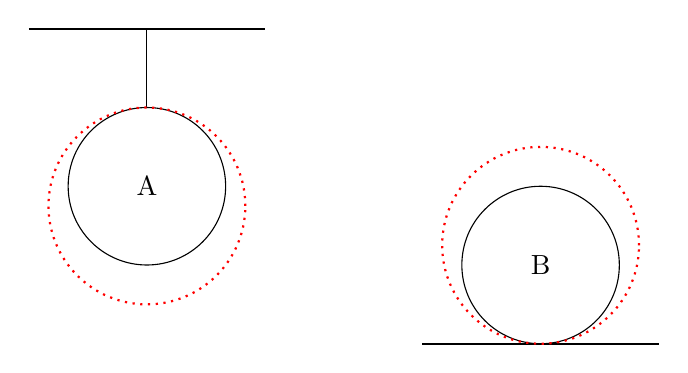
\begin{tikzpicture}
			\draw[thick] (0,4) -- (3,4);
			\draw (1.5,4) -- (1.5,3);
			\draw (1.5,2) circle (1);
			\draw[thick,dotted,red] (1.5,1.75) circle (1.25);
			\draw (1.5,2) node {A};
			\draw[thick] (5,0) -- (8,0);
			\draw (6.5,1) circle (1);
			\draw[thick,dotted,red] (6.5,1.25) circle (1.25);
			\draw (6.5,1) node {B};
		\end{tikzpicture}
		\caption{Auxiliary sketch for Problem 3}
		\label{sketch_3_1}
	\end{figure}
	Displacement of the mass center corresponds to a change of the potential energy of the ball in the gravitational field.\par
	In case of the ball A the potential energy decreases. From the 1$^\text{st}$ principle of thermodynamics, it corresponds to additional heating of the ball.\par
	In case of the ball B the potential energy increases. From the 1$^\text{st}$ principle of thermodynamics it corresponds to some "losses of the heat provided" for performing a mechanical work necessary to rise the ball. The net result is that the final temperature of the ball B should be lower than the final temperature of the ball A.\par
	The above effect is very small. For example, one my find (see later) that for balls made of lead, with radius 10cm, and portion of heat equal to 50kcal, the difference of the final temperature of the balls is of order $10^{-5}$K. For spatial and time fluctuations, such small quantity practically cannot be measured.\par
	Calculation of the dif\mbox{}ference of the f\mbox{}inal temperatures was not required from the participants. Nevertheless, we present it here as an element of discussion.\par
	We may assume that the work against the atmospheric pressure can be neglected. It is obvious that this work is small. Moreover, it is almost the same for both balls. So, it should not affect the dif\mbox{}ference of the temperatures substantially. We will assume that such quantities as specific heat of the lead and coef\mbox{}f\mbox{}icient of thermal expansion of lead are constant (i.e. do not depend on temperature).\par
	The heat used for changing the temperatures of balls may be written as
	\begin{equation*}
		Q_i=mc\Delta t_i\text{, where }i=A\text{ or } B
	\end{equation*}
	Here, $m$ denotes the mass of ball, $c$ the specific heat of lead, and $\Delta t_i$ the change of the temperature of ball.\par
	The changes of the potential energy of the balls are (neglecting signs)
	\begin{equation*}
		\Delta E_i=mgr\alpha\Delta t_i\text{, where }i=A\text{ or }B
	\end{equation*}
	Here, $g$ denotes the gravitational acceleration, $r$ initial radius of the ball, $\alpha$ coef\mbox{}f\mbox{}icient of thermal expansion of lead. We assume here that the thread does not change its length.\par
	Taking into account conditions described in the text of the problem and the interpretation mentioned at the beginning of the solution, we may write
	\begin{IEEEeqnarray*}{c}
		Q=Q_A-\gamma\Delta E_A\\
		Q=Q_B+\gamma\Delta E_B
	\end{IEEEeqnarray*}
	$\gamma$ denotes the thermal equivalent of work $(\approx0.24\frac{\text{cal}}{\text{J}})$. In fact, $\gamma$ is only a conversion ratio between calories and joules. If you use a system of units in which calories are not present, you may omit $\gamma$ at all.\par
	Thus,
	\begin{IEEEeqnarray*}{c}
		Q=(mc-\gamma mgr\alpha)\Delta t_A\text{, for the ball A,}\\
		Q=(mc-\gamma mgr\alpha)\Delta t_B\text{, for the ball B}
	\end{IEEEeqnarray*}
	and
	\begin{equation*}
		\Delta t_A=\frac{Q}{mc-\gamma mgr \alpha}\text{, }\Delta t_B=\frac{Q}{mc+\gamma mgr \alpha}
	\end{equation*}
	Finally, we get
	\begin{equation}
		\Delta t=\Delta t_A-\Delta t_B=\frac{2\gamma gr\alpha}{c^2-(\gamma gr\alpha)^2m}\frac{Q}{m}\approx\frac{2\gamma Qgr\alpha}{mc^2}
	\end{equation}
	We neglected the term with $\alpha^2$ as the coefficient $\alpha$ is very small.\par
	Now we may put the numerical values, $Q=50$kcal, $\gamma=0.24\frac{\text{cal}}{\text{J}}$, $g\approx9.8\text{ms}^{-2}$, $m\approx47$kg (mass of the lad ball with radius equal to 10cm), $r=0.1$m, $c\approx0.031\frac{\text{cal}}{\text{gK}}$, $\alpha\approx29\times10^{-6}\text{K}^{-1}$. After calculations, we get $\Delta t\approx1.5\times10^{-5}$K.
	\subsection*{Problem 4\footnote{The Organizing Committee prepared three theoretical problems. Unfortunately, at the time of the 1$^\text{st}$ Olympiad, the Romanian students from the last class had the entrance examinations at the universities. For that, Romania sent a team consisting of students from younger classes. They were not familiar with electricity. To give them a chance, the Organizers (under agreement of the International Board) added the fourth problem presented here. The student (not only from Romania) were allowed to choose three problems. The maximum possible scores for the problems were: 1$^\text{st}$ problem 10 points, 2$^\text{nd}$ problem 10 points, 3$^\text{rd}$ problem 10 points, and 4$^\text{th}$ problem 6 points. The fourth problem was solved by 8 students. Only four of them solved the problem for 6 points.}}
	A closed vessel with volume $V_0=10l$ contains dry air in the normal conditions ($t_0=0\,^{\circ}\mathrm{C},p_0=1\text{atm}$). In some moment 3g of water were added to the vessel and the system was warmed up to $t=100\,^{\circ}\mathrm{C}$. Find the pressure in the vessel. Discuss assumption you made to solve the problem.\\ \\
	\textbf{Solution}\\
	The water added to the vessel evaporates. Assume that the whole portion of water evaporated. Then the density of water vapor in 100$^{\circ}\mathrm{C}$ should be 0.300$\frac{g}{l}$. It is less than the density of saturated vapor at 100$^{\circ}\mathrm{C}$, which equals to 0.597$\frac{g}{l}$ (The students were allowed to use physical tables). So, at 100$^{\circ}\mathrm{C}$, the vessel contains air and unsaturated water vapor only (without any liquid phase).\par
	Now we assume that both air and unsaturated water vapor behave as ideal gases. In view of Dalton law, the total pressure $p$ in the vessel at 100$^{\circ}\mathrm{C}$ is equal to the sum of partial pressures of the air $p_a$ and unsaturated water vapor $p_v$,
	\begin{equation*}
		p=p_a+p_v
	\end{equation*}\par
	As the volume of the vessel is constant, we may apply the Gay-Lussac law to the air. We obtain
	\begin{equation*}
		p_a=p_0\Big(\frac{273+t}{273}\Big)
	\end{equation*}\par
	The pressure of the water vapor may be found from the equation of state of the ideal gas,
	\begin{equation*}
		\frac{p_vV_0}{273+t}=\frac{m}{\mu}R
	\end{equation*}
	where $m$ denotes the mass of the vapor, $\mu$ the molecular mass of the water and $R$ the universal gas constant. Thus,
	\begin{equation*}
		p_v=\frac{m}{\mu}R\frac{273+t}{V_0}
	\end{equation*}
	and finally
	\begin{equation}
		p=p_0\frac{273+t}{273}+\frac{m}{\mu}R\frac{273+t}{V_0}
	\end{equation}
	Numerically,
	\begin{equation*}
		p=(1.366+0.516)\text{atm}\approx1.88\text{atm}
	\end{equation*}
\section*{Experimental problem}
	\subsection*{Determining Specif\mbox{}ic Heat of Petroleum}
	The following devices and materials are given: 1. Balance (without weights), 2. Calorimeter, 3. Thermometer, 4. Source of voltage, 5. Switches, 6. Wires, 7. Electric heater, 8. Stop-watch, 9. Beakers, 10. Water, 11. Petroleum, 12. Sand (for balancing).\par
	Determine specif\mbox{}ic heat of petroleum. The specif\mbox{}ic heat of water is 1 cal/(g.$^{\circ}\mathrm{C}$). The specif\mbox{}ic heat of the calorimeter is 0.92 cal/(g.$^{\circ}\mathrm{C}$).\par
	Discuss assumptions made in the solution.\\ \\
	\textbf{Solution}\\
	The devices given to the students allowed using several methods. The students used the following three methods:
	\begin{enumerate}
		\item Comparison of velocity of warming up water and petroleum
		\item Comparison of cooling down water and petroleum
		\item Traditional heat balance
	\end{enumerate}\par
	As no weights were given, the students had to use the sand to f\mbox{}ind portions of petrolem and water with masses equal to the mass of calorimeter.\\ \\
	\noindent\emph{First method: comparison of velocity of warming up}\par
	If the heater
\chapter*{II IPhO (Budapest, 1968)}
\addcontentsline{toc}
{chapter}{II IPhO (Budapest, 1968)}
\section*{Theoretical problem}
	\subsection*{Slide and Roll}
	On an inclined plane of 30$^{\circ}$ a block, mass $m_2=4\text{kg}$, is joined by a light cord to a solid cylinder, mass $m_1=8\text{kg}$, radius $r=5\text{cm}$. Find the acceleration if the bodies are released. The coef\mbox{}f\mbox{}icient of friction between the block and the inclined plane $\mu=0.2$. Friction at the bearing and rolling friction are negligible.
	\subsection*{Mixture or Toluene with Dif\mbox{}ferent Temperature}
	There are 300$\text{cm}^3$ toluene of 0$^{\circ}\mathrm{C}$ temperature in a glass and 110$\text{cm}^3$ toluene of 100$^{\circ}\mathrm{C}$ temperature in another glass. Find the final volume after the two liquids are mixed. The coefficient of volume expansion of toluene $\beta=0.001(^{\circ}\mathrm{C})^{-1}$. Neglect the loss of heat.
	\subsection*{Refraction}
	Parallel light rays are falling on the plane surface of a semi-cylinder made of glass, at an angle of 45$^{\circ}$, in such a plane which is perpendicular to the axis of the semi-cylinder. Index of refraction is $\sqrt{2}$. Where are the rays emerging out of the cylindrical surface?
\section*{Experimental problem}
	\subsection*{Mystery boxes}
	Three closed boxes (black boxes) with two plug sockets on each are present for investigation. The participants have to f\mbox{}ind out, without opening the boxes, what kind of elements are in them and measure their characteristic properties. AC and DC meters (their internal resistance and accuracy are given) and AC 50Hz and DC sources are put at the participants' disposal.
\chapter*{III IPhO (Brno, 1969)}
\addcontentsline{toc}
{chapter}{III IPhO (Brno, 1969)}
\section*{Theoretical problem}
	
\section*{Experimental problem}
\chapter*{IV IPhO (Moscow, 1970)}
\addcontentsline{toc}
{chapter}{IV IPhO (Moscow, 1970)}
\chapter*{V IPhO (Sofia, 1971)}
\addcontentsline{toc}
{chapter}{V IPhO (Sofia, 1971)}
\chapter*{VI IPhO (Bucharest, 1972)}
\addcontentsline{toc}
{chapter}{VI IPhO (Bucharest, 1972)}
\chapter*{VII IPhO (Warsaw, 1974)}
\addcontentsline{toc}
{chapter}{VII IPhO (Warsaw, 1974)}
\chapter*{VIII IPhO (G\"ustrow, 1975)}
\addcontentsline{toc}
{chapter}{VIII IPhO (G\"ustrow, 1975)}
\chapter*{IX IPhO (Budapest, 1976)}
\addcontentsline{toc}
{chapter}{IX IPhO (Budapest, 1976)}
\chapter*{X IPhO (Hadrec Kr\'alov\'e, 1977)}
\addcontentsline{toc}
{chapter}{X IPhO (Hadrec Kr\'alov\'e, 1977)}
\chapter*{XI IPhO (Moscow, 1979)}
\addcontentsline{toc}
{chapter}{XI IPhO (Moscow, 1979)}
\chapter*{XII IPhO (Varna, 1981)}
\addcontentsline{toc}
{chapter}{XII IPhO (Varna, 1981)}
\chapter*{XIII IPhO (Malente, 1982)}
\addcontentsline{toc}
{chapter}{XIII IPhO (Malente, 1982)}
\chapter*{XIV IPhO (Bucharest, 1983)}
\addcontentsline{toc}
{chapter}{XIV IPhO (Bucharest, 1983)}
\chapter*{XV IPhO (Sigtuna, 1984)}
\addcontentsline{toc}
{chapter}{XV IPhO (Sigtuna, 1984)}
\chapter*{XVI IPhO (Portoro\v{z}, 1985)}
\addcontentsline{toc}
{chapter}{XVI IPhO (Portoro\v{z}, 1985)}
\chapter*{XVII IPhO (London-Harrow, 1986)}
\addcontentsline{toc}
{chapter}{XVII IPhO (London-Horrow, 1986)}
\chapter*{XVIII IPhO (Jena, 1987)}
\addcontentsline{toc}
{chapter}{XVIII IPhO (Jena, 1987)}
\chapter*{XIX IPhO (Bad Ischl, 1988)}
\addcontentsline{toc}
{chapter}{XIX IPhO (Bad Ischl, 1988)}
\chapter*{XX IPhO (Warsaw, 1989)}
\addcontentsline{toc}
{chapter}{XX IPhO (Warsaw, 1989)}
\chapter*{XXI IPhO (Groningen, 1990)}
\addcontentsline{toc}
{chapter}{XXI IPhO (Groningen, 1990)}
\chapter*{XXII IPhO (Havana, 1991)}
\addcontentsline{toc}
{chapter}{XXII IPhO (Havana, 1991)}
\chapter*{XXIII IPhO (Helsinki-Espoo, 1992)}
\addcontentsline{toc}
{chapter}{XXIII IPhO (Helsinki-Espoo, 1992)}
\chapter*{XXIV IPhO (Williamsburg, 1993)}
\addcontentsline{toc}
{chapter}{XXIV IPhO (Williamsburg, 1993)}
\chapter*{XXV IPhO (Beijing, 1994)}
\addcontentsline{toc}
{chapter}{XXV IPhO (Beijing, 1994)}
\chapter*{XXVI IPhO (Canberra, 1995)}
\addcontentsline{toc}
{chapter}{XXVI IPhO (Canberra, 1995)}

\end{document}